\subsection{Description of the Structures in the Increasing Archetypal Model}
\label{sec:add.add.like}

We start by plotting a 2D period scan of the increasing archetypal model at a corner of the parameter region in between the chains.
Here we changed $b_L$ to $0.8$ and keep $a_L$ and $g_R\left(\frac{1}{2}\right)$, because the period-adding-like structures are more pronounced at these parameter values.
\Cref{fig:add.add.like} shows a 2D period scan with these parameters at a corner of the space between chains.
Here, the parameter region $P^{12}_3$ is in the lower left corner and the parameter region $P^{12}_4$ of the same chain is in the upper right corner.
In the lower right corner is the parameter region $P^{14}_4$.

\begin{figure}
	\centering
	\includegraphics[width=.7 \textwidth]{62_MinimalRepr_Adding/2D_Period_add_zoom/result.png}
	\caption[2D period scan of period-adding-like structures in the increasing archetypal model]{
		2D period scan of period-adding-like structures in the increasing archetypal model.
		The fixed parameters are $a_L = 1, b_L = 0.8,$ and $g_R\left(\frac{1}{2}\right) = \frac{1}{2} + \frac{1}{40}$.
		The parameters $\alpha = g_R\left(\frac{1}{4}\right)$ and $\beta = c_L$ are varied.
	}
	\label{fig:add.add.like}
\end{figure}

\subsubsection{Horizontal Period-adding-like Structures}

\begin{figure}
	\centering
	\subfloat[2D period scan]{
		\includegraphics[width=.45 \textwidth]{62_MinimalRepr_Adding/2D_Period_add_zoom_hor/result.png}
		\label{fig:add.add.like.hor.2D}
	}
	\subfloat[1D period scan]{
		\includegraphics[width=.45 \textwidth]{62_MinimalRepr_Adding/1D_Period_hor_low/result.png}
		\label{fig:add.add.like.hor.1D}
	}
	\caption[2D and 1D period scans of horizontal period-adding-like structures in the increasing archetypal model]{
		2D and 1D period scans of horizontal period-adding-like structures in the increasing archetypal model.
		The fixed parameters are $a_L = 1, b_L = 0.8,$ and $g_R\left(\frac{1}{2}\right) = \frac{1}{2} + \frac{1}{40}$.
		(a) shows the 2D period scan where the parameters $\alpha = g_R\left(\frac{1}{4}\right)$ and $\beta = c_L$ are varied.
		The small arrow indicates the parameter range for the 1D period scan in (b).
		Here, only $\beta$ is varied.
		The numbers at the top mark the periods at the corresponding value for $\beta$.
	}
	\label{fig:add.add.like.hor}
\end{figure}

\subsubsection{Vertical Period-adding-like Structures}

\begin{figure}
	\centering
	\subfloat[2D period scan]{
		\includegraphics[width=.45 \textwidth]{62_MinimalRepr_Adding/2D_Period_add_zoom_vert/result.png}
		\label{fig:add.add.like.vert.2D}
	}
	\subfloat[1D period scan]{
		\includegraphics[width=.45 \textwidth]{62_MinimalRepr_Adding/1D_Period_vert_left/result.png}
		\label{fig:add.add.like.vert.1D}
	}
	\caption[2D and 1D period scans of vertical period-adding-like structures in the increasing archetypal model]{
		2D and 1D period scans of vertical period-adding-like structures in the increasing archetypal model.
		The fixed parameters are $a_L = 1, b_L = 0.8,$ and $g_R\left(\frac{1}{2}\right) = \frac{1}{2} + \frac{1}{40}$.
		(a) shows the 2D period scan where the parameters $\alpha = g_R\left(\frac{1}{4}\right)$ and $\beta = c_L$ are varied.
		The small arrow indicates the parameter range for the 1D period scan in (b).
		Here, only $\alpha$ is varied.
		The numbers at the top mark the periods at the corresponding value for $\alpha$.
	}
	\label{fig:add.add.like.vert}
\end{figure}

\subsubsection{Period-adding-like Structures in the Corners}

\begin{figure}
	\centering
	\subfloat[2D period scan]{
		\includegraphics[width=.45 \textwidth]{62_MinimalRepr_Adding/2D_Period_add_zoom_corn/result.png}
		\label{fig:add.add.like.corn.2D}
	}
	\subfloat[1D period scan]{
		\includegraphics[width=.45 \textwidth]{62_MinimalRepr_Adding/1D_Period_corn_vert/result.png}
		\label{fig:add.add.like.corn.1D}
	}
	\caption[2D and 1D period scans of period-adding-like structures in the corners of the spaces between chains in the increasing archetypal model]{
		2D and 1D period scans of the period-adding-like structures in the corners of the spaces between chains in the increasing archetypal model.
		The fixed parameters are $a_L = 1, b_L = 0.8,$ and $g_R\left(\frac{1}{2}\right) = \frac{1}{2} + \frac{1}{40}$.
		(a) shows the 2D period scan where the parameters $\alpha = g_R\left(\frac{1}{4}\right)$ and $\beta = c_L$ are varied.
		The big arrow indicates the parameter range for the 1D period scan in (b).
		Here, only $\alpha$ is varied.
		The numbers at the top mark the periods at the corresponding value for $\alpha$.
	}
	\label{fig:add.add.like.corn}
\end{figure}

The 1D period scan in \Cref{fig:add.add.like.corn.1D} of the vertical scan across the structure in the corner of the space between the chains with period $12$ and $14$ looks similar to the 1D period scan in \Cref{fig:add.add.like.vert.1D} of the vertical period-adding-like structure.
\todo{Basically the same structure, describe}
\todo{Find citation where similar thing was found \cite{tramontana2012period}}

\todo{old:}

We start by plotting the periods of stable cycles in a one-dimensional scan across a period-adding structure.
\Cref{fig:minrep.adding1.motivation.halved.1d.period.full} shows this scan, while \Cref{fig:minrep.adding1.corner.period.full} shows the period-structure.
The period range on the one-dimensional scan is marked in red between the regions $P_{10}^4$ and $P_{10}^4 \oplus P_9^4$.
The regions $P_{10}^4$ and $P_9^4$ have cycles as we expect, $\Cycle{\A^6\B^4\C^6\D^4}$ and $\Cycle{\A^5\B^4\C^5\D^4}$.
But the region $P_{10}^4 \oplus P_9^4$ is weirder.
In this region, there are two coexisting cycles, that act like the coexisting cycles in ``type B'' parameter regions.
They are hybrids of the cycles $P_{10}^4$ and $P_9^4$, $\Cycle{\A^6\B^4\C^5\D^4}$ and $\Cycle{\A^5\B^4\C^6\D^4}$, acting like one cycle on the one half of the model and acting like the other cycles on the other half.
This is the first sign, that there is something off about this period-adding structure.

Examining the one-dimensional scan of the period-adding structure, \Cref{fig:minrep.adding1.motivation.halved.1d.period.full}, closer we find some inconsistencies.
First, the period of the cycle $\sigma\rho$, 58, is larger than the periods of $\sigma$, 20, and $\rho$, 19, combined.
This is unexpected because the cycle $\sigma\rho$ should be the cycles $\sigma$ and $\rho$ glued together, and therefore its period should be exactly the sum of the periods of the cycles $\sigma$ and $\rho$.
Similarly, the period of $\sigma^2\rho$ should be the sum of the periods of $\sigma$ and $\sigma\rho$.
But instead, the period of $\sigma^2\rho$ is smaller than the period of $\sigma\rho$.
Is this not a period-adding cascade after all?

What is happening here is that a period-adding structure in the halved model manifests as this weird structure in the full model.
This becomes apparent when simulating the halved model in the same period ranges.
\Cref{fig:minrep.adding1.motivation.halved.1d.period.halved} shows the one-dimensional period scan in the halved model that corresponds to the scan in the full model in \Cref{fig:minrep.adding1.motivation.halved.1d.period.full}.
In the halved model, $\sigma$ is the cycle $\Cycle{\L^6\R^4}$, which is expected for the cycle $P_{10}^4$, and $\rho$ is the cycle $\Cycle{\L^6\R^4\L^5\R^4}$.
The cycle $\sigma\rho$ in between the two is now actually the two cycles glued together $\Cycle{(\L^6\R^4)^2\L^5R^4}$, as we would expect in a period-adding structure.
And its period is 29, which is the sum of the periods of the cycle $\sigma$, 10, and $\rho$, 19.

Now we can also see that the unusual hybrid cycles $P_{10}^4 \oplus P_9^4$ in the full model are the manifestation of the cycle $\Cycle{L^6\R^4\L^5\R^4}$ in the halved model.
This cycle is itself the first level of the real period-adding structure of the cycles $P_{10}^4$ and $P_9^4$, which are $\Cycle{\L^6\R^4}$ and $\Cycle{L^5\R^4}$ in the halved model.
\Cref{fig:minrep.adding1.large.adding} shows a one-dimensional scan of a full period-adding structure in the halved model at different parameter values that allow for larger period regions with higher periods, making them visible to us.
In the next section, we will explain what exactly the halved model is, why it works in our case, and how to translate symbolic sequences between it and the full model.

\begin{figure}
	\centering
	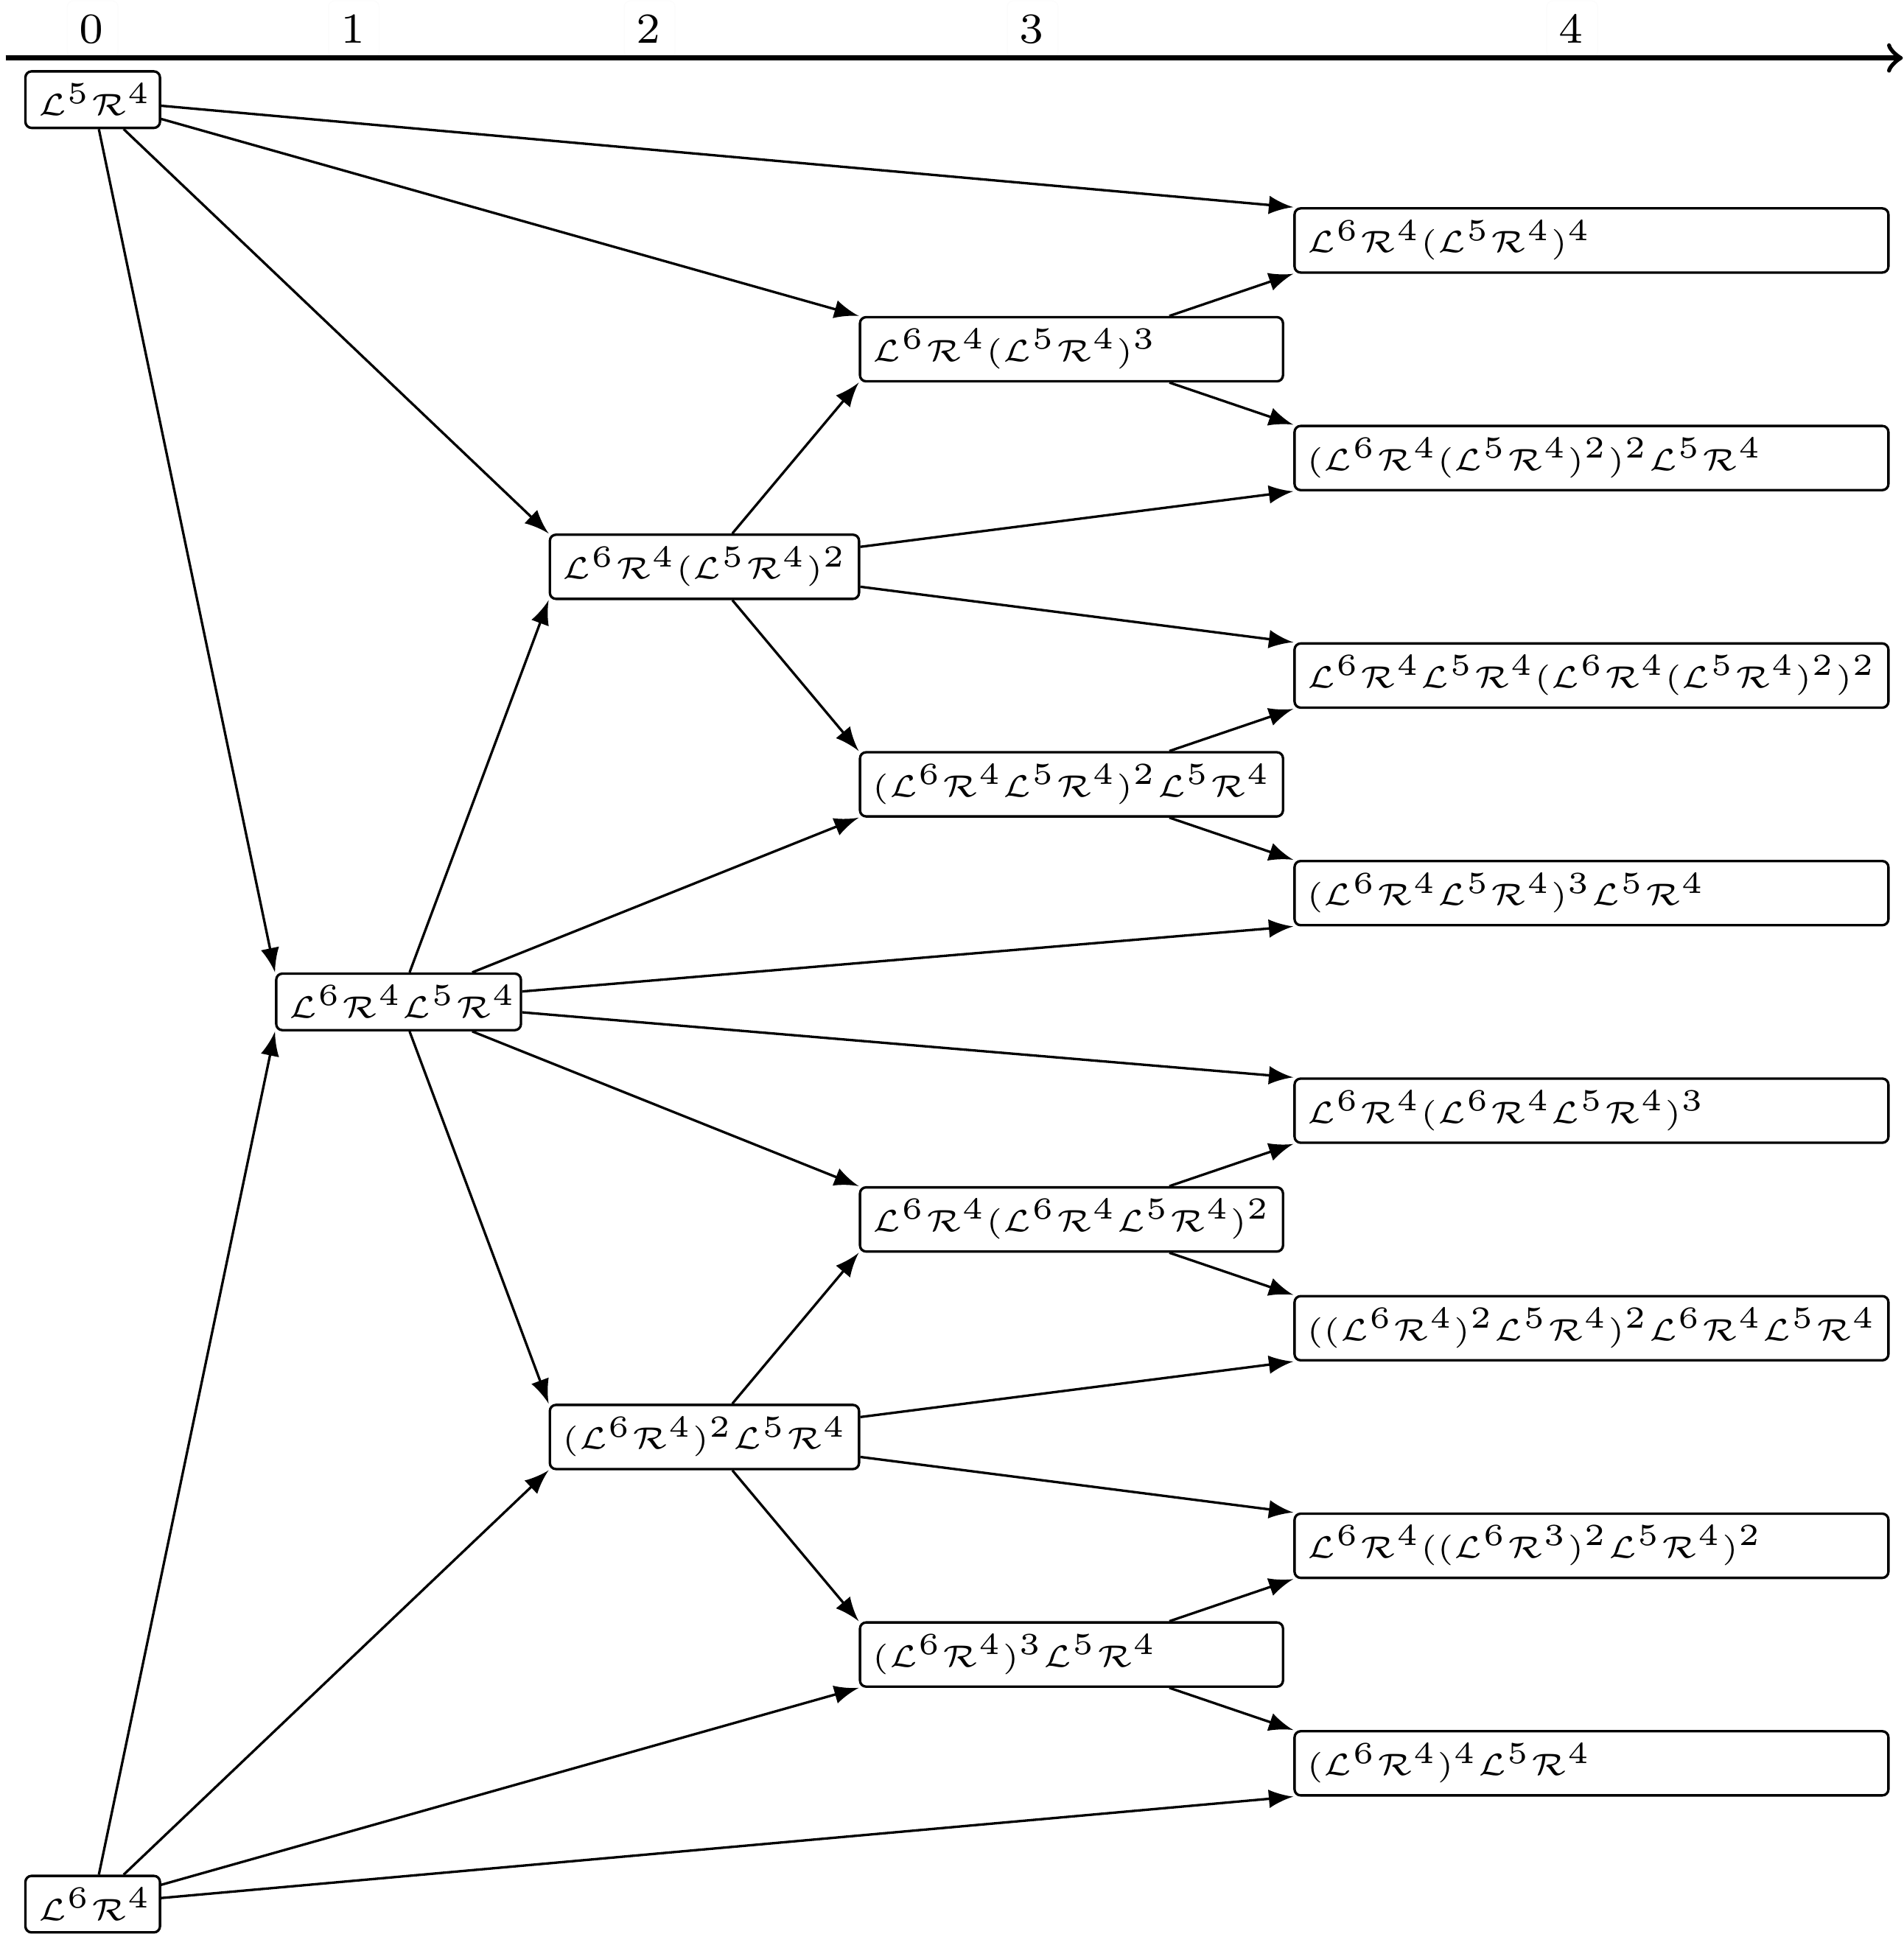
\includegraphics[width=\textwidth]{FareyTrees/Minrep_Adding1_Full/adding.png}
	\caption{t}
	\label{fig:tree.adding1.hor.full}
\end{figure}
